%%\documentclass[aip,jcp]{revtex4-1}
\documentclass[aip
, pra
, showpacs
, aps
, twocolumn
%, onecolumn
, groupedaddress
, floatfix
%, preprint
]{revtex4}
%]{revtex4-1}
\usepackage{graphicx, amsbsy, bm, dcolumn, amsmath}

\newcommand{\etal}{{\em et~al.\/}}
\newcommand{\beq}{\begin{equation}}
\newcommand{\eeq}{\end{equation}}
\newcommand{\barr}{\begin{array}}
\newcommand{\earr}{\end{array}}
\newcommand{\vecr}{{\bf r}}
\newcommand{\dd}{\mbox{d}}
\newcommand{\dr}{\mbox{d} r}
\newcommand{\vare}{\varepsilon}
\newcommand{\calN}{{\cal N}}
\newcommand{\di}{_{\mbox{\tiny{di}}}}
\newcommand{\ex}{_{\mbox{\tiny{ex}}}}



\newcommand{\isum}%
{\mathop{\hbox{$\displaystyle\sum\kern-13.2pt\int\kern1.5pt$}}}

\begin{document}

\title {Electron-helium $S$-wave scattering. II. Single ionization and single excitation}

\author{Dmitry A. Konovalov}
\affiliation{Discipline of Information Technology, School of Business}
\affiliation{ARC Centre for Antimatter-Matter Studies, James Cook University, Townsville, Queensland 4811, Australia}

\author{Dmitry V. Fursa}
\affiliation{ARC Centre for Antimatter-Matter Studies,
Curtin University, GPO Box U1987, Perth, Western Australia 6845, Australia}

\author{Igor Bray}
\affiliation{ARC Centre for Antimatter-Matter Studies,
Curtin University, GPO Box U1987, Perth, Western Australia 6845, Australia}



\date{\today}

\begin{abstract}

In the preceding paper (referred as Ref. [I]), [D. A. Konovalov {\em et. al.} Phys. Rev. A {\bf 84}, 032707 (2011)],
the $S$-wave $e$-He scattering problem was solved within the frozen-core (FC) model of helium for
the elastic, $2^{1,3}S$-excitation, and single ionization cross sections for impact energies in the range 0.1-1000eV.
The reported in Ref. [I] "proof-of-principle" J-matrix (JM) calculations were in complete agreement with the convergent-close-coupling (CCC) method,
which was also applied to the FC model.
In this sequel, the target helium atom is described at much higher level of accuracy by disregarding the FC model.
Both target electrons are described within the configuration-interaction (CI) model of helium obtaining accurate
first seven bound states of helium.
It is found that the theory in Ref. [I] is sufficient to solve the $S$-model for single-excitation and single-ionization.
The presented JM results (0.1-1000 eV) are confirmed by the corresponding CCC calculations providing
total elastic, $2^{1,3}S$ and $3^{1,3}S$ excitation cross sections with a "benchmark"-level of accuracy for the first time for the considered $S$-wave model.

\end{abstract}

\pacs{34.80.Dp} %34.80.Dp	Atomic excitation and ionization
\maketitle



\section{INTRODUCTION}

Resonances in electron-atom scattering processes is a striking quantum mechanical phenomenon, which were comprehensively reviewed by \citet{Schulz73} in 1973 and then by \citet{BC94} in 1994.
Historically and limiting the scope of this introduction to the helium and atomic hydrogen scattering targets, in 1962 \citet{BS62} theoretically predicted a very sharp resonance in the elastic $e$-H scattering  at 9.6~eV with a half-width ($\Gamma$) of 0.1~eV. Due to technical difficulties working with atomic hydrogen, the resonances were confirmed experimentally first for the $e$-He scattering, when in 1963 \citet{Schulz63} observed the resonance in the elastic $e$-He scattering at 19.3~eV with $\Gamma$=0.06~eV.
Since their discovery in the 1960s, the resonances have been and continue to be studied extensively
for $e$-H \cite{WC94,FRA94_pra,KM94pL741,OSB95p4320,DLTL96,DTLM99,DTL00} and $e$-He \cite{KM95pL139,HBSBB96,NP01,PN03,SMC2006} (citing only studies not already referenced in \cite{Schulz73,BC94}),
where it is well understood that the resonances are nothing more (nor less) than the manifestation of the negative-ion metastable states \cite{BC94}.


This study focuses on the resonances in the $S$-wave $e$-He ($S$-$e$-He) scattering,
where the target helium atom is in its ground state before the electron impact,
and where only the partial wave with zero angular momentum ($l=0$) is retained in all calculations
and partial-wave expansions.
The $S$-wave model has proven to be a very productive testing ground for scattering theories,
see \cite{T62,HY74p1209,P78,P80,P81,CO84,BS92p53,BST93,KM94pL407,IDHF95,PS96,JS02,JS00l,BRIM99,S99l,MHR02,BS04,Frapiccini10} for the $S$-wave $e$-H scattering ($S$-$e$-H)
and \cite{DHIF94,PMR99,PBFS02,PNBFS04,HMR05R,HMR05,BS10p022715,BS10p022716,KFB11} for  the $S$-$e$-He problem.
The main attraction of the $S$-wave model is that it retains most of the physics complexities of the full
scattering problems while simplifying the problems computationally.
In particular, it is somewhat expected or implied that if a theoretical method solves the $S$-wave model, then
the remaining partial waves could be solved with additional computational resources, which is in deed the case for the CCC \cite{FB95} and JM \cite{KM94pL741,KM95pL139} methods.


The main goal of this study is to provide high accuracy total elastic and excitation $S$-$e$-He cross sections below the ionization threshold, focusing on their resonant features.
The need for such benchmark theoretical data is evident from the existing {\em ab initio} attempts to solve the $S$-$e$-He problem.
Reviewing in reverse chronological order, in 2010 \citet{BS10p022715} developed a four-body propagating exterior scaling (PECS) method and reported results claiming to achieve "benchmark" level of accuracy.
However none of their cross sections, including elastic and $2^{1,3}S$ excitation cross sections, displayed any resonances at the accuracy level achieved for the $S$-$e$-H problem \cite{P78}.
In 2005, \citet{HMR05} reported results using
time-dependent exterior complex scaling (TD-ECS), which also failed to described resonance behavior of the cross sections.
The notable exception is the convergent-close-coupling (CCC) method which in 2002 and 2004 \cite{PBFS02,PNBFS04}
did not examine the resonance regions with sufficiently fine energy grid.
This is now corrected to some extent when in 2011 \citet{KFB11} reported the CCC and $J$-matrix (JM) {\em frozen-core}
(FC) results clearly showing the resonances in the elastic and $n=2$ ($2^1S$ and $2^3S$) excitation cross sections.


The stated goal is achieved by applying the CCC method together with the JM method,
where the later has been recently revised by merging it with the Fano's multi-configuration interaction matrix elements \cite{Fano65},
see \cite{JMatrixWebsite} for information on availability of the JM source code used in this paper.

\begin{table}[htb]
\caption{\label{Tab_ENGS}
Energies and classifications for $S$-wave helium electron configurations.
Energies $e_i$  and $E_i$ are from Eqs.~(\ref{psi_H_psi}) and (\ref{Psi_from_Fano}), respectively.
$\lambda_{\rm L}=4$, $N_c=N_t$
}
\begin{ruledtabular}
%\begin{tabular}{lcr}
\begin{tabular}{llll}
Classification & threshold & $e_i$  &    \\
\hline
                      &    & -2.879 028 767 315 &  Ref. \cite{G94}    \\
                      &    & -2.879 028 732   &  Ref. \cite{JB97p2614}    \\
$\mbox{He}(1s^2,^1S)$ &  0 & -2.879 028 569 1 &  $N_t=50$   \\ %-2.879028569120921, -2.1441972587315763, -2.060794037546864,
                      &    & -2.879 028 504   &  $N_t=45$   \\
                      &    & -2.879 027 69    &  Ref. \cite{DHIF94}    \\
                      &    & -2.879 03        &  Ref. \cite{HMR05R}    \\
                      &    & -2.878 95        &  Ref. \cite{BS10p022715}    \\
\hline
$\mbox{He}(1s2s,^3S)$    & 0.704 763 712  & -2.174 264 856 2 & $N_t=50$ \\  %-2.174264856287701, -2.0684901366080752,
                         &                & -2.174 264 856 2 & $N_t=45$ \\
\hline
$\mbox{He}(1s2s,^1S)$    & 0.734 831 310 & -2.144 197 258 7 &  $N_t=50$ \\
                         &               & -2.144 197 253   &  $N_t=45$   \\
\hline
$\mbox{He}(1s3s,^3S)$    & 0.810 538 432 & -2.068 490 136 6 & $N_t=50$  \\
                         &               & -2.068 490 135   & $N_t=45$\\
\hline
$\mbox{He}(1s3s,^1S)$    & 0.818 234 531 & -2.060 794 037 5 & $N_t=50$ \\
                         &               & -2.060 794 025   & $N_t=45$\\
\hline
$\mbox{He}(1s4s,^3S)$    & 0.842 589 989 & -2.036 438 58    & Ref. \cite{DHIF94} \\
\hline
$\mbox{He}^+(1s)$        & 0.879 028 569 & -2 	 &    \\
\end{tabular}
\end{ruledtabular}
\end{table}


\begin{figure}[htb]
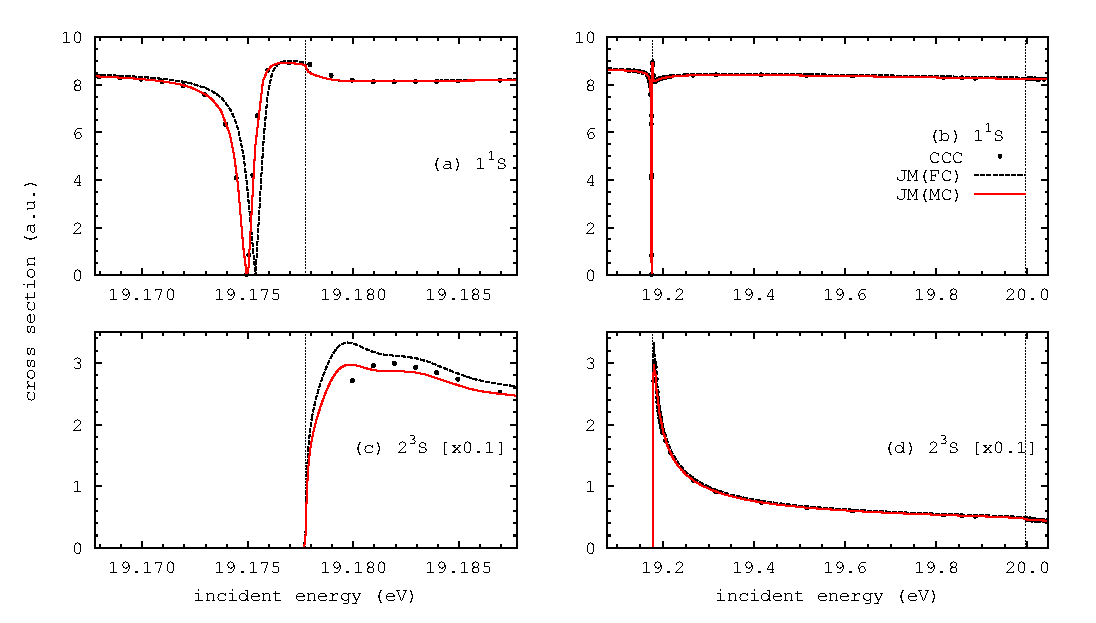
\includegraphics[scale=0.9]{fig1.ps}
\caption{(Color online) Elastic ($1^1S$),
single $n=2$ excitation ($2^3S$ and $2^1S$) and single ionization cross sections ($\sigma_{\mbox{\tiny{I}}}$) for electron scattering on a ground-state helium target in
the $S$-wave model.}
\label{Fig_TICS}
\end{figure}


\begin{figure}[htb]
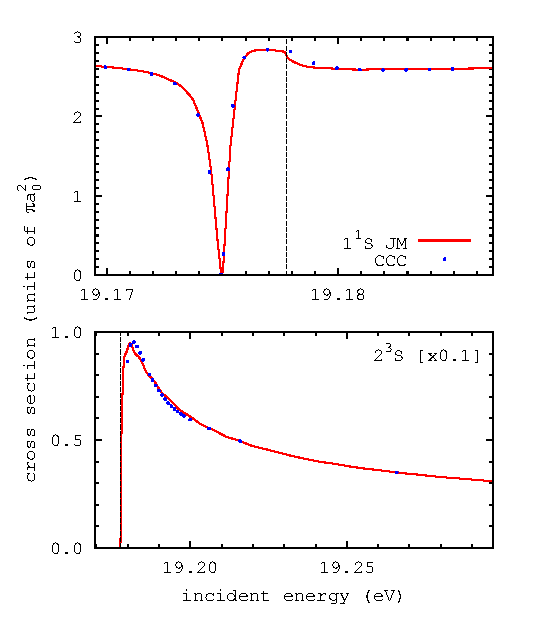
\includegraphics[scale=1]{fig_res_1S_2S3.ps}
\caption{(Color online)
The same as in Fig.~\ref{Fig_TICS}
but zooming in on the $2^3S$ excitation threshold (Table~\ref{Tab_ENGS}) shown by the vertical dashed line.
}
\label{Fig_2S3}
\end{figure}


\begin{figure}[htb]
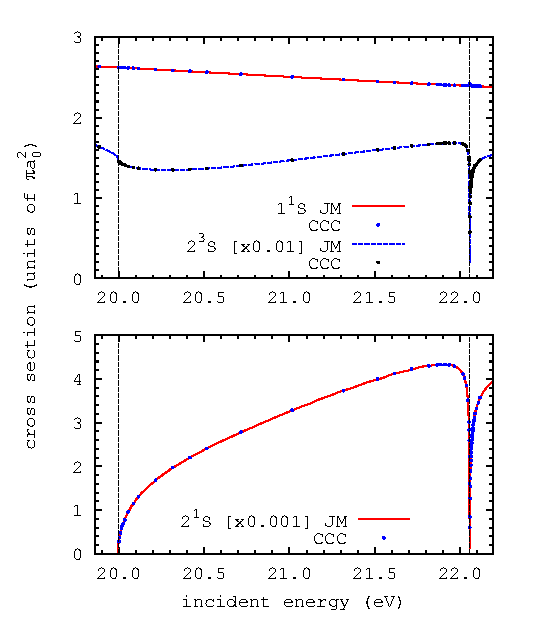
\includegraphics[scale=1]{fig_res_2S1.ps}
\caption{(Color online) The same as in Fig.~\ref{Fig_TICS}
but for the impact energies between the $2^1S$ and $3^3S$ excitation thresholds (Table~\ref{Tab_ENGS}) shown by the left and right vertical dashed lines, respectively.
}
\label{Fig_2S1}
\end{figure}


\begin{figure}[htb]
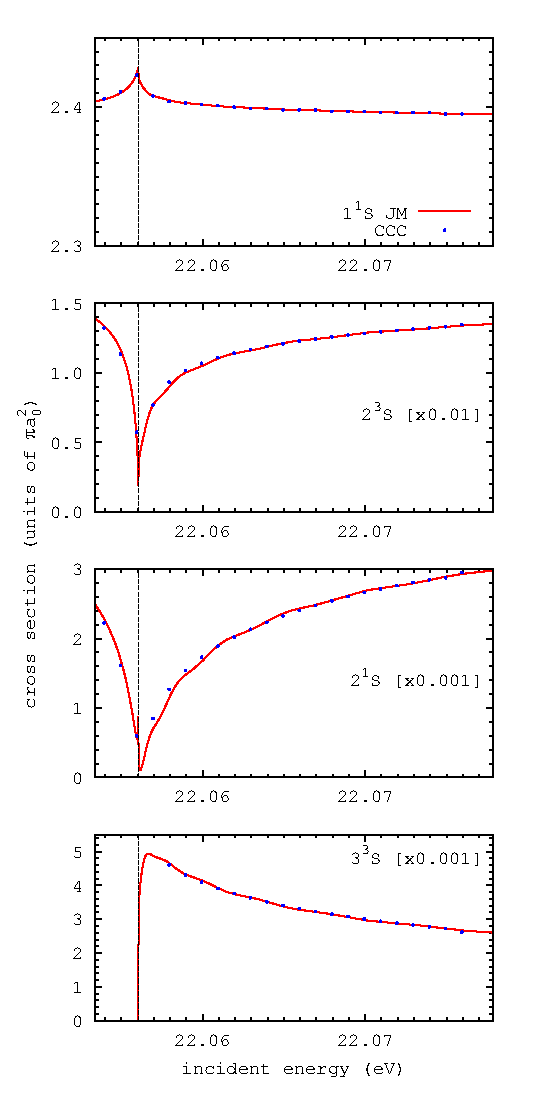
\includegraphics[scale=1]{fig_res_3S3.ps}
\caption{(Color online) The same as in Fig.~\ref{Fig_2S3}
but zooming in on the $3^3S$ excitation threshold (Table~\ref{Tab_ENGS}).
}
\label{Fig_3S3}
\end{figure}


\begin{figure}[htb]
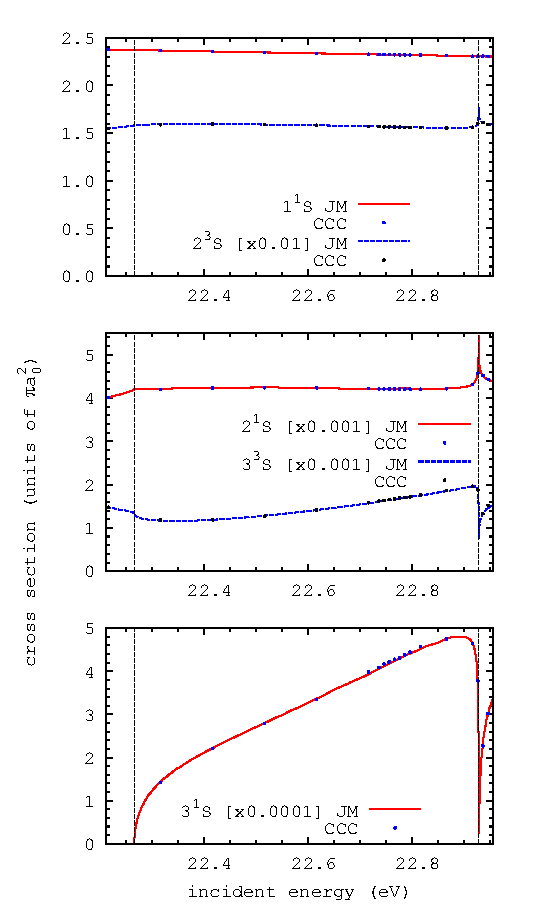
\includegraphics[scale=1]{fig_res_3S1.ps}
\caption{(Color online) The same as in Fig.~\ref{Fig_2S1}
but for the impact energies between the $3^1S$ and $4^3S$ excitation thresholds (Table~\ref{Tab_ENGS}).
}
\label{Fig_3S1}
\end{figure}





\section{THEORY}

\subsection{Wave functions}
TODO: describe two Laguerre bases.

Let the nonorthogonal Laguerre functions used in the original JM method \cite{HY74p1201,BR76p1491}
be referred to as the JM functions and denoted by $\{\xi_p(r)\}_{p=0}^\infty$,
\[
\xi_p(r) = x^{l+1} \mbox{e}^{-x /2}
L_p^{2l+1}(x), \ \ \ p = 0, 1, ..., \infty,
\]
where $x=\lambda_{\rm L} r$,  $\lambda_{\rm L}$ is the Laguerre exponential falloff,
$l \equiv 0$ (for the $S$-model), and $L_p^{\alpha}(x)$ are the associated Laguerre polynomials \cite{abramowitz}.
The JM method splits the one-electron radial functional space into {\em inner} $\{\xi_p\}_{p=0}^{N-1}$
and {\em outer} $\{\xi_p\}_{p=N}^\infty$
subsets controlled by the number ($N$) of JM functions in the inner subset \cite{HY74p1201,BR76p1491}.




\section{RESULTS}

\subsection{Resonances in $e$-He $S$-wave scattering}


[TODO]
Atomic unit of energy (or Hartree) was set to 27.2116 eV. A tabular
form of the JM and CCC cross sections is available from jmatrix.googlecode.com .



Again, both CCC and JM methods described the target helium atom
, where the target eigenstates were constructed from the first $N_t$ JM functions (\ref{psi_H_psi}). Convergence in the CCC cross sections
(Figs.~\ref{Fig_He_n2} and \ref{Fig_He_n3}) was achieved at $N_t=?$, where the corresponding JM cross sections
converged at $N_t=?$ and $N=?$.






\section{CONCLUSIONS}





\begin{acknowledgments}
This work was supported by the Australian Research Council. IB
acknowledges the Australian National Computational Infrastructure
Facility and its Western Australian node iVEC.
\end{acknowledgments}



\bibliographystyle{apsrev}
\bibliography{../bibtex/qm_references}

\end{document}
